\subsection{In-depth Semi-structured Interviews}

From all of the twenty interviews, fifteen people preferred the personalised
itineraries and gave valid reasons. However, three out of the people who
selected the non-personalised itinerary stated that they think their social
media presence does not reflect their travel preferences.


%\paragraph{Inidividual one}:  
%The first interviewee had the following traits: personal characteristics:
%enjoys shopping, nightlife and clubbing. Since they do not like to miss out on
%any POIs of a site, they chose to generate a fast-paced activity plan $C = 3$ for
%seven days $M = 7$. Person one is active on social media and posts frequently on
%social media. The application gathered 100 preferences from this person, and
%table ~\ref{indOne} shows their generated travel interest vector.
									
%The first timetable shown was the non-personalised itinerary, and they made the
%following points:

%\begin{table}[h]
%\caption{Travel Interest Vector of Individual One} \label{t:tab}

%\centerline{
  %\begin{tabular}{|l|c|c|c|c|c|} 
 %\hline
      %Beach & Museums	& Nature	& Shops & Clubs & Bars \\
 %\hline
      %1.32\% & 4.35\%	& 4.61\%	& 89.47\% & 69.23\% &30.77\%\\
 %\hline
  %\end{tabular}
%}
%\label{indOne}
%\end{table}

%\begin{itemize}
%\item Initially, they thought the timetable was quite personalised since it tried to capture a balance of POIs of a different category and thought this reflected their lifestyle.
%\item They were satisfied with the travel time between the places making it very doable.
%\item They felt that the timetable included too many cultural places and stated that they would change about 40\% of the timeline if they had to follow it strictly and spend more time shopping.
%\item They rated the itinerary as 'quite personalised' and were 'very satisfied'.
%\end{itemize}

%The following are comments from the second itinerary, i.e. the personalised one:
%\begin{itemize}
%\item The interviewee changed their opinion immediately and figured out this was the personalised solution since the first day was a day dedicated to shopping. 
%\item Since the timetable included more natural locations, they felt that this was the appealing itinerary and would stick with 95\% of this plan.
%\item The suggested places were all places that the person has been to recently.
%\item The evening places were very appealing since it includes a lot of the best night clubs.
%\item They rated the itinerary as 'very personalised' and were 'very satisfied'.
%\end{itemize}
%When shown their automatically generated preferences, person one felt that the
%'beach' category should be higher, and the rest was very accurate. In addition, person one deemed this approach ideal since it gives an in-depth itinerary for a tourist, which is also ideal to discover new places.


%\paragraph{Individual two}: 

%When travelling, the second individual searches for a relaxed holiday with a
%mix of beaches and the main tourist attractions. Therefore, they chose to
%generate a moderate activity plan $C=2$ for five days $M=5$.Furthermore, person two thinks
%that their social media presence represents their travel preferences since they
%post numerous pictures when they travel. The application gathered ten pictures
%and liked pages from their profile, and table ~\ref{inTwo} shows the generated preferences.


%\begin{table}[h]
%\caption{Travel Interest Vector of Individual Two} \label{t:tab}

%\centerline{
  %\begin{tabular}{|l|c|c|c|c|c|} 
 %\hline
      %Beach & Museums	& Nature	& Shops & Clubs & Bars \\
 %\hline
      %50\% & 20\%	& 25\%	& 0\% & 0\% &100\%\\
 %\hline
  %\end{tabular}
%}
%\label{inTwo}
%\end{table}

%The first timetable shown was the
%non-personalised itinerary, and they made the following points:
%\begin{itemize}
%\item The holiday is structured very well and reflects their potential travel plan since there is a resting time between the evening activities and a place to eat right after.
%\item They were unsure whether the first itinerary is personalised since they usually spend more time at the beach and less time in Museums.
%\item There are too many clubs in the evening and would personally go to more bars and relaxed places.
%\item They rated this itinerary `not very personalised' but rated 'satisfied' overall. 

%\end{itemize}
%The following are comments from the second itinerary, i.e. the personalised one:
%\begin{itemize}
%\item This itinerary is more personalised since there are more beaches and natural places.
%\item The evenings are more adapted since there are more places to sit down, drink, and chat than clubbing venues.
%\item This itinerary was rated `very personalised' and `very satisfied' overall. 
%\end{itemize}

%After the second itinerary, we discussed the travel interest vector with the
%interviewee. They stated that they would leave their characteristics the same,
%however, switch the shopping category with museums which are preferential. They
%mentioned that the museums category score is a quite high since they like to
%view science-related locations to keep up to date but the number of museums
%presented was deemed to be too high compared to their likings. Six other
%interviewees also mentioned that their ’museums’ characteristic was rated high.

%To further personalise the itinerary, person two suggested that the algorithm
%should also look at the photos posted by the people they follow online since it
%would gather much more information. 

%To personalise the itinerary further, person two suggested that the algorithm
%should also include photos posted by people they follow online, since it would
%gather more information, making the itinerary more accurate.

%\paragraph{Person Three}: When travelling, they tend to look for places with a
%lot of nature and cultural sightseeing. In addition, this person is very
%interested in music and art, so they also like to travel to art galleries and
%museums.  Person three likes to make the most out of their holiday, so they
%chose to generate a fast-paced $C=3$ six-day itinerary $M=6$. However, they don't think
%their social media profile represents what they would look for in a holiday. As
%a result, the application only gathered ten items, and their preferences are as
%follows:

%The first result shown to this person was the personalised itinerary, and
%they made the following conclusions: 

%\begin{table}[h]
%\caption{Travel Interest Vector of Individual Three} \label{t:tab}

%\centerline{
  %\begin{tabular}{|l|c|c|c|c|c|} 
 %\hline
      %Beach & Museums	& Nature	& Shops & Clubs & Bars \\
 %\hline
      %42.86\% & 9.09\%	& 23.81\%	& 23.81\% & 50\% & 50\%\\
 %\hline
  %\end{tabular}
%}
%\label{inTwo}
%\end{table}

%\begin{itemize} 
    %\item They would enjoy
    %less nightlife and more relaxed activities in the evening.  
    %\item They would prefer 
    %more natural sights along with the museums such as hikes and walks around
    %the environment.  
    %\item They felt that the timetable was not very personalised.
    %\end{itemize} 

%From the non-personalised itinerary, person three made the
%following conclusions:

%\begin{itemize} \item They felt that this timetable was more balanced 
%and appropriate.  \item Since it included more
%nature-related places, it felt more personalised.  \end{itemize}

\begin{figure}[h]
\centering
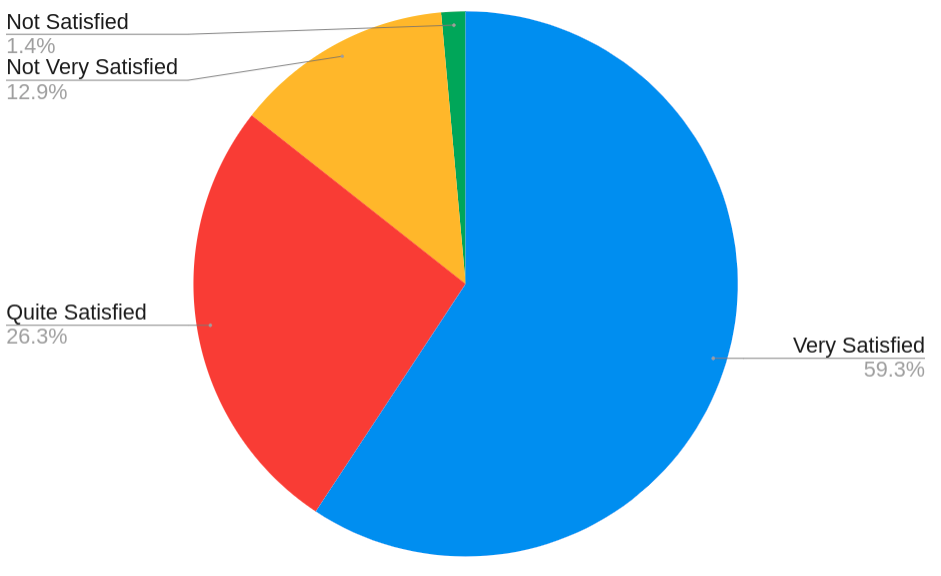
\includegraphics[width=0.34\textwidth]{xiHaga.png}
\caption{Satisfaction Rating of The Gathered Characteristics.}
\label{Satisfaction}
\end{figure}

From all of the interviews it was noted that the more active a person
is on social media, the more accurate the characteristics are which leads to a more accurate 
travel itinerary. In fact, figure ~\ref{Satisfaction}  shows that most of the
preferences gathered, belong to users who felt very satisfied with the overall results.



